% !TEX TS-program = lualatex
\documentclass{beamer}
\input{../common/misomva}
\newcommand{\misoclasstinytitleslide}{Partially based on material by:  Ulrike von Luxburg, \\[-1em] Gary Miller, Doyle \& Schnell, Daniel Spielman}
\newcommand{\misoclassdate}{}
\usetikzlibrary{graphs}

\begin{document}

% Topic-specific title slide
\newcommand{\topictitle}{Similarity Graphs Construction}
\newcommand{\topicsubtitle}{Building Graphs from Data}
\MakeTopicSlide

\begin{frame}
\frametitle{Similarity Graphs}

Input: $\bx_1, \bx_2,\bx_3, \dots, \bx_\nodes $
\begin{itemize}
\item
raw data 
\item
flat data
\item
vectorial data
\end{itemize}

\begin{center}

\includegraphics[width=0.6\columnwidth]{../img/movies1}
\end{center}

\end{frame}
%%%%%%%%%%%%%%%%%%%%%%%%%%%%%%%%%%%%%%%%%%%%%%%%%%%%%%%%%%%%%
%%%%%%%%%%%%%%%%%%%%%%%%%%%%%%%%%%%%%%%%%%%%%%%%%%%%%%%%%%%%%
\begin{frame}
\frametitle{Similarity Graphs}

Similarity graph: $\cG = (\nodeset, \edgeset)$ ---  \textbf{(un)weighted}

\begin{block}{}
\emph{Task 1:} For each pair $i$, $j$: define a \textbf{similarity function} $s_{ij}$\\ \smallskip
\emph{Task 2:} Decide which edges to include
\end{block}
\pause
\begin{description}
\item[fully connected graphs] - consider everything 
\item[$\varepsilon$-neighborhood graphs]  -- connect the points with the distances smaller than $\varepsilon$ 
\item[$k$-NN neighborhood graphs] -- take $k$ nearest neighbors 
\end{description}
\pause

\emph{This is art (not much theory exists).}

{\scriptsize 
\url{http://www.informatik.uni-hamburg.de/ML/contents/people/luxburg/publications/Luxburg07_tutorial.pdf}
}

\end{frame}
%%%%%%%%%%%%%%%%%%%%%%%%%%%%%%%%%%%%%%%%%%%%%%%%%%%%%%%%%%%%%
\begin{frame}
\frametitle{Similarity Graphs: Fully connected graphs}
\begin{block}{}
Edges connect everything.
\end{block}
\pause
\begin{itemize}%\addtolength{\itemsep}{0.4\baselineskip}
\item choose a ``meaningful'' similarity function $s$  
\item default choice: \[s_{ij} = \exp\left(\frac{ -\| \bx_i - \bx_j\|^2}{2\sigma^2} \right) \]
\item \questionbox{why the exponential decay with the distance?}
\pause
\item $\sigma$ controls the width of the neighborhoods
\begin{itemize}
%\item similar role as $\varepsilon$
\item \textbf{a} practical rule of thumb: 10\% of the average empirical std 
\item possibility: learn  $\sigma_i$ for each feature independently
\end{itemize}
\item metric learning (a whole field of ML)
\end{itemize}
\end{frame}
%%%%%%%%%%%%%%%%%%%%%%%%%%%%%%%%%%%%%%%%%%%%%%%%%%%%%%%%%%%%%
\begin{frame}
\frametitle{Similarity Graphs: $\varepsilon$-neighborhood graphs}

\begin{block}{}
Edges connect the points with the distances smaller than $\varepsilon$.
\end{block}
\only<1>{\begin{center}
\begin{figure}[!h]
    \centering
    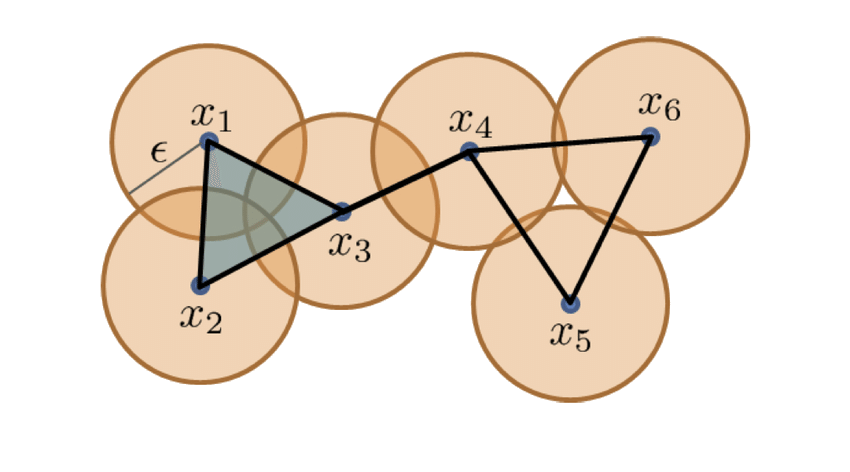
\includegraphics[scale=.2]{../img/chain_complex.png}
    \caption{An $\varepsilon$-graph. {\tiny Source: Illustration of a Rips complex}}
\end{figure}
\end{center}}
\only<2->{\begin{itemize}%\addtolength{\itemsep}{0.75\baselineskip}
\item distances are roughly on the same scale $(\varepsilon)$ 
\item weights may not bring additional info $\to$ unweighted
\item equivalent to: similarity function is at least $\varepsilon$
\item theory [Penrose, 1999]:  $\varepsilon = ((\log \nodes)/\nodes)^d$ to guarantee connectivity 
{\tiny $\nodes$ nodes, $d$ dimension} 
\item practice: choose $\varepsilon$ as the length of the longest edge in the MST - minimum spanning tree
\end{itemize}
\pause
\rightquestionbox{What could be the problem with this MST approach?} 
\pause
\onslide<handout:0>{
\rightyellbox{Anomalies can make $\varepsilon$ too large.}}}

\end{frame}
%%%%%%%%%%%%%%%%%%%%%%%%%%%%%%%%%%%%%%%%%%%%%%%%%%%%%%%%%%%%%
\begin{frame}
\frametitle{Similarity Graphs: $k$-nearest neighbors  graphs}
\begin{block}{}
Edges connect each node to its $k$-nearest neighbors.
\end{block}
\pause
\begin{itemize}\addtolength{\itemsep}{0.4\baselineskip}
\item asymmetric (or directed graph) 
\begin{itemize}
\item option OR: ignore the direction
\item option AND: include if we have both direction (mutual $k$-NN)  
\end{itemize}
\item \questionbox{how to choose $k$?} 
\item $k \approx \log \nodes$ - suggested by asymptotics (practice: up to $\sqrt{\nodes}$)
\item for mutual $k$-NN we need to take larger $k$
\item mutual $k$-NN does not connect regions with different density 
\item \questionbox{why don't we take $k = \nodes - 1$?}
\onslide<handout:0>{
\begin{itemize}
\item
space and time 
\item 
manifold considerations (preserving local properties)
\end{itemize}}
\end{itemize}
\end{frame}
%%%%%%%%%%%%%%%%%%%%%%%%%%%%%%%%%%%%%%%%%%%%%%%%%%%%%%%%%%%%%
\begin{frame}
\frametitle{Similarity Graphs: Important considerations}

\begin{itemize}[<+-| alert@+>]%\addtolength{\itemsep}{0.75\baselineskip}
\item \emph{calculate all $s_{ij}$ and threshold} has its limits ($\nodes \approx 10000$)  
\item graph construction step can be a huge bottleneck
\item want to go higher? (we often have to)
\begin{itemize}
\item down-sample
\item approximate NN 
\begin{itemize}
\item \textbf{LSH} - Locally Sensitive Hashing
\item \textbf{CoverTrees} 
%\item \textbf{Spectral sparsifiers} 
\end{itemize}
\item sometime we may not need the graph (just the final results)
\item yet another story: when we start with a large graph and want to make it sparse (later in the course)
\end{itemize}
\item these rules have little theoretical underpinning 
\item similarity is very data-dependent 
\end{itemize}
\end{frame}

\MakeLastSlide
\end{document}
